%Version 2.1 April 2023
% See section 11 of the User Manual for version history
%
%%%%%%%%%%%%%%%%%%%%%%%%%%%%%%%%%%%%%%%%%%%%%%%%%%%%%%%%%%%%%%%%%%%%%%
%%                                                                 %%
%% Please do not use \input{...} to include other tex files.       %%
%% Submit your LaTeX manuscript as one .tex document.              %%
%%                                                                 %%
%% All additional figures and files should be attached             %%
%% separately and not embedded in the \TeX\ document itself.       %%
%%                                                                 %%
%%%%%%%%%%%%%%%%%%%%%%%%%%%%%%%%%%%%%%%%%%%%%%%%%%%%%%%%%%%%%%%%%%%%%

%%\documentclass[referee,sn-basic]{sn-jnl}% referee option is meant for double line spacing

%%=======================================================%%
%% to print line numbers in the margin use lineno option %%
%%=======================================================%%

%%\documentclass[lineno,sn-basic]{sn-jnl}% Basic Springer Nature Reference Style/Chemistry Reference Style

%%======================================================%%
%% to compile with pdflatex/xelatex use pdflatex option %%
%%======================================================%%

%%\documentclass[pdflatex,sn-basic]{sn-jnl}% Basic Springer Nature Reference Style/Chemistry Reference Style


%%Note: the following reference styles support Namedate and Numbered referencing. By default the style follows the most common style. To switch between the options you can add or remove “Numbered” in the optional parenthesis. 
%%The option is available for: sn-basic.bst, sn-vancouver.bst, sn-chicago.bst, sn-mathphys.bst. %  
 
%%\documentclass[sn-nature]{sn-jnl}% Style for submissions to Nature Portfolio journals
%%\documentclass[sn-basic]{sn-jnl}% Basic Springer Nature Reference Style/Chemistry Reference Style
%%\documentclass[sn-mathphys,Numbered]{sn-jnl}% Math and Physical Sciences Reference Style
%%\documentclass[sn-aps]{sn-jnl}% American Physical Society (APS) Reference Style
%%\documentclass[sn-vancouver,Numbered]{sn-jnl}% Vancouver Reference Style
%%\documentclass[sn-apa]{sn-jnl}% APA Reference Style 
%%\documentclass[sn-chicago]{sn-jnl}% Chicago-based Humanities Reference Style
\documentclass[default]{sn-jnl}% Default
%%\documentclass[default,iicol]{sn-jnl}% Default with double column layout

%%%% Standard Packages
%%<additional latex packages if required can be included here>

\usepackage{graphicx}%
\usepackage{multirow}%
\usepackage{amsmath,amssymb,amsfonts}%
\usepackage{amsthm}%
\usepackage{mathrsfs}%
\usepackage[title]{appendix}%
\usepackage{xcolor}%
\usepackage{textcomp}%
\usepackage{manyfoot}%
\usepackage{booktabs}%
\usepackage{algorithm}%
\usepackage{algorithmicx}%
\usepackage{algpseudocode}%
\usepackage{listings}%
%%%%

%%%%%=============================================================================%%%%
%%%%  Remarks: This template is provided to aid authors with the preparation
%%%%  of original research articles intended for submission to journals published 
%%%%  by Springer Nature. The guidance has been prepared in partnership with 
%%%%  production teams to conform to Springer Nature technical requirements. 
%%%%  Editorial and presentation requirements differ among journal portfolios and 
%%%%  research disciplines. You may find sections in this template are irrelevant 
%%%%  to your work and are empowered to omit any such section if allowed by the 
%%%%  journal you intend to submit to. The submission guidelines and policies 
%%%%  of the journal take precedence. A detailed User Manual is available in the 
%%%%  template package for technical guidance.
%%%%%=============================================================================%%%%

%\jyear{2021}%

%% as per the requirement new theorem styles can be included as shown below
% \theoremstyle{thmstyleone}%
% \newtheorem{theorem}{Theorem}%  meant for continuous numbers
% %%\newtheorem{theorem}{Theorem}[section]% meant for sectionwise numbers
% %% optional argument [theorem] produces theorem numbering sequence instead of independent numbers for Proposition
% \newtheorem{proposition}[theorem]{Proposition}% 
% %%\newtheorem{proposition}{Proposition}% to get separate numbers for theorem and proposition etc.

% \theoremstyle{thmstyletwo}%
% \newtheorem{example}{Example}%
% \newtheorem{remark}{Remark}%

% \theoremstyle{thmstylethree}%
% \newtheorem{definition}{Definition}%

\raggedbottom
%%\unnumbered% uncomment this for unnumbered level heads

\begin{document}

\title[AskVerse]{AskVerse – Secure, Scalable, and Real-time Knowledge Management using RAG and Multi-Agent Framework}

%%=============================================================%%
%% Prefix	-> \pfx{Dr}
%% GivenName	-> \fnm{Joergen W.}
%% Particle	-> \spfx{van der} -> surname prefix
%% FamilyName	-> \sur{Ploeg}
%% Suffix	-> \sfx{IV}
%% NatureName	-> \tanm{Poet Laureate} -> Title after name
%% Degrees	-> \dgr{MSc, PhD}
%% \author*[1,2]{\pfx{Dr} \fnm{Joergen W.} \spfx{van der} \sur{Ploeg} \sfx{IV} \tanm{Poet Laureate} 
%%                 \dgr{MSc, PhD}}\email{iauthor@gmail.com}
%%=============================================================%%

\author*[1]{\fnm{Manoj} \sur{Chavan}}\email{chavan.manoj@gmail.com}

\affil*[1]{\orgdiv{Technology Department}, \orgname{Kotak Bank Ltd}, \orgaddress{\city{Bengaluru}, \postcode{560066}, \state{Karnataka}, \country{India}}}

%%==================================%%
%% sample for unstructured abstract %%
%%==================================%%

\abstract{Traditional Retrieval-Augmented Generation (RAG) based systems face significant limitations in handling structured, multi-source knowledge retrieval, particularly within complex enterprise environments where information is dispersed across documents, APIs, intranet systems, and dynamic web sources. Existing solutions often lack robust query decomposition, real-time adaptability, and mechanisms for conveying confidence in responses, thereby diminishing their utility in critical decision-making scenarios.

This paper introduces AskVerse, a novel system built upon a multi-agent architecture meticulously optimized for secure, scalable, and real-time knowledge management. Key innovations embedded within AskVerse include: \textbf{Chain-of-Thought Reasoning}, which systematically decomposes complex user queries into structured sub-queries; \textbf{Multi-Agent Orchestration}, employing specialized agents to intelligently retrieve and synthesize knowledge from a diverse array of enterprise sources such as internal websites, proprietary documents, enterprise APIs, Confluence, academic research papers, and real-time web searches. The system further enhances retrieval efficacy through a \textbf{Hybrid Search Mechanism} that integrates dense retrieval (utilizing OpenAI embedding), sparse retrieval (based on BM25), and sophisticated ensemble search techniques for superior relevance. To address the critical aspect of trustworthiness, AskVerse incorporates \textbf{Uncertainty Quantification} by providing explicit citations alongside generated responses. AskVerse implements robust \textbf{Security and Data Privacy measures} including fine-grained access control, data masking protocols, and comprehensive document citation tracking to address stringent enterprise demands. Furthermore, dedicated \textbf{Performance Measurement and Optimization} tooling is integrated for RAGAs-based evaluation, systematic benchmarking of retriever and generator components and continuous improvement of recall metrics. This system culminates in a flexible, \textbf{plug-and-play} architecture that facilitates seamless integration of new APIs, vector databases, and advanced retrieval techniques, all while upholding high standards of accuracy, security, and transparency.
}

%%================================%%
%% Sample for structured abstract %%
%%================================%%

% \abstract{\textbf{Purpose:} The abstract serves both as a general introduction to the topic and as a brief, non-technical summary of the main results and their implications. The abstract must not include subheadings (unless expressly permitted in the journal's Instructions to Authors), equations or citations. As a guide the abstract should not exceed 200 words. Most journals do not set a hard limit however authors are advised to check the author instructions for the journal they are submitting to.
% 
% \textbf{Methods:} The abstract serves both as a general introduction to the topic and as a brief, non-technical summary of the main results and their implications. The abstract must not include subheadings (unless expressly permitted in the journal's Instructions to Authors), equations or citations. As a guide the abstract should not exceed 200 words. Most journals do not set a hard limit however authors are advised to check the author instructions for the journal they are submitting to.
% 
% \textbf{Results:} The abstract serves both as a general introduction to the topic and as a brief, non-technical summary of the main results and their implications. The abstract must not include subheadings (unless expressly permitted in the journal's Instructions to Authors), equations or citations. As a guide the abstract should not exceed 200 words. Most journals do not set a hard limit however authors are advised to check the author instructions for the journal they are submitting to.
% 
% \textbf{Conclusion:} The abstract serves both as a general introduction to the topic and as a brief, non-technical summary of the main results and their implications. The abstract must not include subheadings (unless expressly permitted in the journal's Instructions to Authors), equations or citations. As a guide the abstract should not exceed 200 words. Most journals do not set a hard limit however authors are advised to check the author instructions for the journal they are submitting to.}

\keywords{AskVerse, RAG, Multi-agent, plugnplay}

%%\pacs[JEL Classification]{D8, H51}

%%\pacs[MSC Classification]{35A01, 65L10, 65L12, 65L20, 65L70}

\maketitle
\sloppy

\section{Introduction}\label{sec1}

Traditional RAG systems, while powerful for static knowledge bases, frequently fall short in scenarios demanding access to real-time data from operational APIs. This inherent limitation curtails their ability to provide up-to-the-minute insights crucial for dynamic business operations. Concurrently, while Agentic AI offers promising avenues for dynamic data access and intelligent task execution, its deployment in enterprise settings introduces significant concerns regarding security vulnerabilities, regulatory compliance, and overall system control. Enterprises face a unique set of challenges in adopting AI for their real-time knowledge management:

\begin{enumerate}
    \item \textbf{Gap with Real-Time Data} - Traditional RAG systems are fundamentally designed to operate on static or periodically updated knowledge bases. They inherently lack the capability to seamlessly integrate and utilize real-time enterprise data streamed from dynamic systems and operational APIs. This limitation severely restricts their ability to provide current insights, rendering them less effective in scenarios where up-to-the-minute information is paramount.
    \item \textbf{Risks Associated with Agentic AI} - While the concept of Agentic AI offers promising avenues for dynamic data access and autonomous task execution, its deployment in enterprise settings introduces considerable risks. These risks primarily revolve around security vulnerabilities, ensuring regulatory compliance, and maintaining predictable control over system behavior. Unchecked agent capabilities can lead to data breaches, non-compliance, and unpredictable operational outcomes, thereby making such systems inherently vulnerable and unpredictable without proper safeguards.
    \item \textbf{Inefficient Query Handling} - Retrieving comprehensive information from a multitude of diverse sources necessitates sophisticated query planning, intelligent sequencing of operations and coherent collation of results. Conventional RAG pipelines often prove inadequate in their ability to effectively decompose complex, multi-faceted user queries into meaningful and executable sub-queries. This deficiency frequently results in inefficient information retrieval, leading to incomplete or inaccurate responses.
    \item \textbf{Lack of Uncertainty Awareness} - A critical deficiency in most existing knowledge retrieval systems is their inability to explicitly indicate the confidence levels associated with their generated responses or to provide clear source citations. Without such transparency, users find it exceedingly difficult to assess the reliability and trustworthiness of the information provided, particularly when making high-stakes decisions. This absence of uncertainty awareness can lead to misinformed judgments and erode user confidence in the system.
    \item \textbf{Fragmented Information Retrieval} - Enterprises typically house information across a wide spectrum of formats and locations – from structured databases and internal documents to external web pages and real-time feeds. Existing models struggle to effectively prioritize, rank, and consolidate relevant information from these diverse knowledge sources. The challenge lies in synthesizing these disparate pieces into a cohesive and contextually accurate response that directly addresses the user's query or action.
    \item \textbf{Security \& Access Control Issues} - Enterprise data, especially sensitive or proprietary information, mandates stringent permission-aware retrieval mechanisms. Many general-purpose RAG systems lack the sophisticated security infrastructure required to enforce fine-grained access control, implement data masking for sensitive attributes, or manage data handling in compliance with corporate policies and regulatory mandates. This poses significant risks of unauthorized data exposure or misuse.
    \item \textbf{Limited Scalability \& Integration} - The dynamic nature of modern enterprises implies a continuous evolution of their technology stacks, including the addition of new APIs and the expansion of knowledge bases. Traditional RAG pipelines often exhibit rigid architectures that do not offer the necessary plug-and-play capability to seamlessly integrate with these ever-growing enterprise APIs and evolving data landscapes. This limits their long-term scalability and adaptability.
\end{enumerate}

Collectively, these inherent limitations lead to a fundamental problem: inconsistent, unreliable, and potentially insecure knowledge retrieval within enterprise environments. This directly impacts operational efficiency, decision-making quality, and overall organizational agility.

\section*{Literature Survey}
To establish a comprehensive understanding of the current state-of-the-art, identify existing gaps, and contextualize the contributions of AskVerse, a thorough literature survey was conducted across several pertinent domains:

\begin{enumerate}
    \item \textbf{Retrieval-Augmented Generation (RAG)} - Studies in this area consistently highlight the transformative efficacy of RAG systems in enhancing the accuracy and factual grounding of generative models. By integrating a retrieval component that fetches relevant information from external knowledge bases before text generation, RAG mitigates issues like hallucination and improves response fidelity compared to standalone LLMs. Key research explores various retriever architectures (e.g., dense vs. sparse), indexing strategies, and fusion techniques for integrating retrieved documents with the generative model~\cite{ref1}. However, much of the existing work primarily focuses on open-domain knowledge and often overlooks the specific complexities of proprietary, heterogeneous, and real-time enterprise data sources.
    \item \textbf{Knowledge Management Systems (KMS)} - Traditional knowledge management solutions have focused on structuring, storing, and disseminating organizational information. These systems typically involve document management and collaboration platforms. While effective for static knowledge repositories, existing KMS platforms largely lack dynamic integration capabilities with advanced generative AI models, emphasizing the need for innovative approaches~\cite{ref2,ref3}.
    \item \textbf{Challenges in Enterprise AI Adoption} - Research into the adoption of AI technologies, particularly LLMs, within enterprise environments reveals a consistent set of significant hurdles. These include, but are not limited to, stringent data privacy regulations, the inherent complexity of integrating AI systems with legacy IT infrastructure and diverse data sources, and the necessity for domain-specific adaptability and fine-tuning~\cite{ref4,ref5}. This body of literature underscores the critical need for enterprise AI solutions that prioritize security, compliance, and flexible integration while delivering domain-relevant accuracy.
    \item \textbf{Advances in Large Language Models (LLMs)} - Recent advancements in LLMs have showcased their extraordinary capabilities in natural language understanding, generation, and complex reasoning. Models like GPT-3, GPT-4, and their derivatives have demonstrated proficiency in tasks ranging from summarization and translation to question answering and creative writing. However, the literature also delineates their inherent limitations, particularly concerning their reliance on pre-trained data, their potential for ``hallucination,'' and their challenges in directly accessing and reasoning over proprietary, real-time, or frequently updated enterprise information not present in their training corpora~\cite{ref6}.
    \item \textbf{Chain-of-Thought Reasoning} - Chain-of-Thought (CoT) prompting has emerged as a powerful technique to enhance the complex reasoning capabilities of LLMs. By explicitly eliciting intermediate reasoning steps, CoT helps models break down multistep problems, improving performance on tasks requiring arithmetic, commonsense reasoning, and symbolic manipulation. While existing CoT approaches often leverage linear reasoning chains, the complexities of enterprise queries frequently demand more sophisticated reasoning structures, such as hierarchical decomposition, conditional branching, or iterative loops until a definitive answer is converged upon~\cite{ref7}. This survey identifies a gap in applying more dynamic and adaptive CoT mechanisms to enterprise knowledge retrieval.
    \item \textbf{Multi-Agent Systems} - The literature on Multi-Agent Systems (MAS) demonstrates their effectiveness in distributed problem-solving and task coordination. Each agent can be designed with specific expertise (e.g., database querying, web scraping, and document analysis) and access to distinct data sources. By distributing tasks and coordinating their efforts, MAS improves overall retrieval accuracy, response coherence, and system adaptability in dynamic environments. Research in this area explores agent communication protocols, task allocation, and conflict resolution mechanisms, with a particular focus on developing security-aware orchestration frameworks for sensitive enterprise contexts~\cite{ref8}.
    \item \textbf{Uncertainty Quantification (UQ) in LLMs} - Uncertainty Quantification in LLMs is an increasingly vital research area aimed at developing methodologies to assess and communicate the confidence levels in generated responses. Current research explores various UQ techniques, including probabilistic methods, Bayesian approaches, and ensemble techniques. The objective is to provide transparent indicators of response reliability, often through confidence scores or explicit source attribution~\cite{ref9}.
    \item \textbf{Evaluation frameworks} - The evaluation of enterprise knowledge management systems, especially those incorporating generative AI, requires comprehensive frameworks that go beyond traditional metrics. Such frameworks must account for factors like relevance, accuracy, completeness, timeliness, security, compliance, and user satisfaction. This survey examines existing evaluation methodologies, including those adapted for RAG systems (e.g., RAGAs-based metrics like faithfulness, answer relevance, context recall, context precision) and general enterprise AI system performance benchmarks. The identified gap lies in establishing standardized, holistic evaluation frameworks tailored specifically for the unique operational and security requirements of enterprise knowledge management solutions leveraging multi-agent RAG~\cite{ref10}.
\end{enumerate}

\section*{Proposed System}
AskVerse is designed as a secure, scalable, and real-time knowledge management system, fundamentally transforming how enterprises interact with their vast and diverse information repositories. At its core, AskVerse employs a sophisticated multi-agent architecture coupled with advanced retrieval and generation techniques to deliver precise, contextually relevant, and trustworthy responses.

AskVerse distinguishes itself through several key innovations:
\begin{enumerate}
    \item \textbf{Chain-of-Thought Reasoning} - This foundational component enables AskVerse to process complex, multi-faceted user queries by breaking them down into a series of structured, logical sub-queries. This systematic decomposition ensures that even the most intricate information needs are addressed methodically, leading to more accurate and comprehensive responses.
    \item \textbf{Multi-Agent Orchestration} - AskVerse leverages a network of specialized agents, each designed with specific expertise and access to distinct knowledge sources. These agents intelligently coordinate their efforts to retrieve, analyze, and synthesize information from a heterogeneous array of enterprise data, including internal enterprise reports (PDFs), intranet websites, APIs etc.
    
    This orchestration ensures that information is retrieved from the most relevant and authoritative sources, regardless of format or location.
    \item \textbf{Hybrid Search Mechanism} - To maximize retrieval relevance and recall, AskVerse integrates a sophisticated hybrid search strategy. This mechanism combines Dense Retrieval (Utilizes advanced embedding e.g., OpenAI embedding), Sparse Retrieval (traditional keyword-based methods like BM25 for efficient and precise matching of exact terms), and Ensemble Retrieval (using fusion techniques, to achieve superior overall relevance and coverage).
    \item \textbf{Uncertainty Quantification} - To foster trust and transparency, AskVerse provides explicit citations and source attribution alongside its generated responses. This allows users to verify the provenance of information, assess its reliability, and understand the confidence level associated with the answer.
    \item \textbf{Security \& Data Privacy} - Recognizing the paramount importance of data security in enterprise environments, AskVerse incorporates robust measures, including:
    \begin{itemize}
        \item Access Control - Implements fine-grained, permission-aware access mechanisms to ensure that users can only retrieve information they are authorized to view.
        \item Data Masking - Automatically identifies and masks sensitive data (e.g., credit card numbers, national identification numbers) within responses to prevent accidental exposure.
        \item Document Citation Tracking - Maintains a traceable log of all documents and sources used in generating a response, facilitating auditing and compliance.
    \end{itemize}
    \item \textbf{Performance Measurement \& Optimization} - AskVerse is equipped with dedicated tooling for continuous monitoring and improvement of its performance. This includes:
    \begin{itemize}
        \item RAGAs-based Evaluation - Utilizes metrics from the RAGAs framework (e.g., faithfulness, answer relevance, context recall, context precision) to quantitatively assess the quality of responses.
        \item Retriever/Generator Benchmarking - Provides tools to systematically evaluate the performance of individual retrieval and generation components.
    \end{itemize}
\end{enumerate}

The proposed architecture of AskVerse offers modularity, resilience, and efficient processing of knowledge queries, as depicted in Figure~\ref{fig:architecture}. The architecture leverages a structured pipeline from user query to tailored response.

\begin{figure}
    \centering
    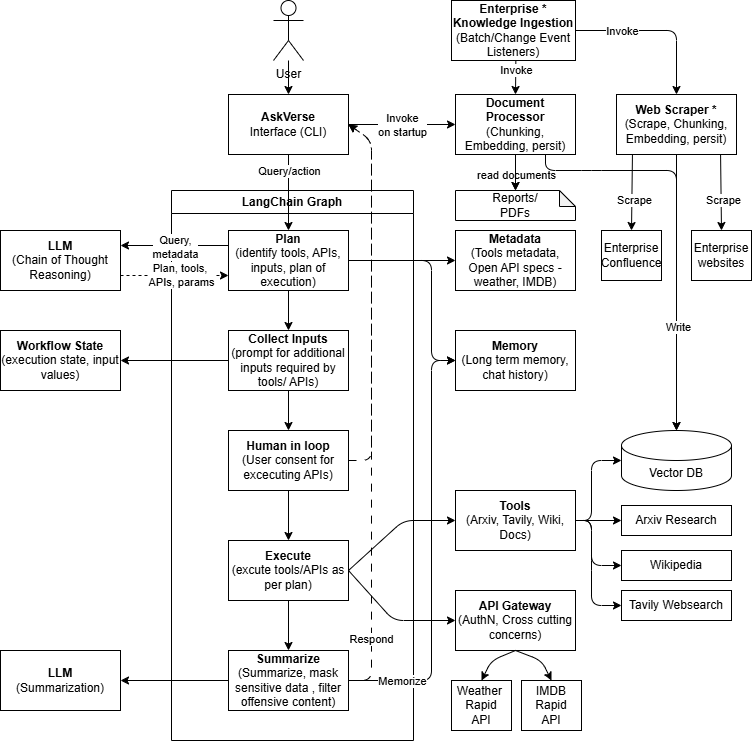
\includegraphics[width=1\linewidth]{design.png}
    \caption{AskVerse Architecture Diagram}
    \label{fig:architecture}
\end{figure}

\section*{Evaluation}
The AskVerse system's performance and effectiveness are rigorously evaluated using a comprehensive framework, with a primary focus on the RAGAs framework. This framework provides quantitative metrics to assess the quality of responses generated by Retrieval-Augmented Generation (RAG) pipelines, focusing on key aspects relevant to knowledge management.

\subsection*{Metrics used for evaluation}
Table~\ref{tab1} explains the metrics used to test the performance of Retriever and Generator components of AskVerse.
\begin{table}[h]
\caption{Evaluation metrics}\label{tab1}%
\renewcommand{\arraystretch}{1.2}
\setlength{\tabcolsep}{4pt}
\begin{tabular}{|p{2.5cm}|p{2cm}|p{4cm}|p{4cm}|}
\hline
\textbf{Metric} & \textbf{Component} & \textbf{Description} & \textbf{Depends on} \\
\hline
Context Precision & Retriever & Measures the proportion of relevant chunks in the retrieved contexts. & Question, Retrieved contexts \\
\hline
Context Recall & Retriever & How many of the relevant documents (or pieces of information) were successfully retrieved. It focuses on not missing important results. & Reference answer, Retrieved contexts \\
\hline
Context Entity Recall & Retriever & Measure of what fraction of entities is recalled from reference. & Entities defined in Reference answer and Retrieved contexts. \\
\hline
Faithfulness & Generator & Measures how factually consistent a response is with the retrieved context. & Question, Retrieved contexts and the Generated answer \\
\hline
Answer Relevancy & Generator & Measures the relevance of the answer to the question. & Question, Generated answer \\
\hline
\end{tabular}
\end{table}

\subsection*{Types of questions used for evaluation}
Table~\ref{tab2} explains the types of questions used to test the performance of AskVerse.
\begin{table}[h]
\caption{Types of questions used for evaluation}\label{tab2}%
\renewcommand{\arraystretch}{1.2}
\setlength{\tabcolsep}{4pt}
\begin{tabular}{|p{2cm}|p{3.5cm}|p{3.5cm}|p{3.5cm}|}
\hline
\textbf{Question Category} & \textbf{Description} & \textbf{How it evaluates RAG Pipeline} & \textbf{Example} \\
\hline
Simple & These are straightforward fact-based queries. & They check if the RAG pipeline can retrieve and generate correct information. & What sustainable innovations has Google introduced in cloud services? \\
\hline
Reasoning & These require logical thinking or inference. & They test if the RAG pipeline can connect information correctly. & Why does IPC Section 4 extend to acts committed outside India? \\
\hline
Multi-context & These need multiple pieces of retrieved information to generate a response. & They evaluate how well the model retrieves and merges different sources. & How does Google compare to Microsoft in renewable energy usage? \\
\hline
\end{tabular}
\end{table}

\subsection*{Evaluation Methodology}
The evaluation methodology for AskVerse is designed to systematically assess both the individual components and the end-to-end performance of the RAG pipeline, leveraging the RAGAs framework and complementary benchmarking tools.

\begin{enumerate}
    \item \textbf{Test Dataset Generation} - To conduct a robust evaluation, a high-quality test dataset is generated. This dataset comprises a list of questions and their corresponding reference answers. The test questions are designed to cover various categories – simple, reasoning and multi-context, as described in Table 2. These test datasets can be generated in two ways - by supplying raw documents to the RAGAs framework's tooling for automatic question generation, or by handcrafting them to ensure specific complexities and coverage of different query types.
    \item \textbf{RAG Query Execution and Capture} - For each question in the loaded test dataset, the AskVerse RAG pipeline is queried. The system's complete response is captured, which includes the generated answer and the specific retrieved context (documents or chunks) that were used to formulate that answer. This also includes any citations provided by AskVerse.
    \item \textbf{RAGAs-based Metrics Calculation} - The questions, reference answers, generated answers and retrieved contexts are then fed into the RAGAs framework for automated evaluation. The RAGAs framework computes these metrics as described in Table~\ref{tab1} – Context precision, Context Recall, Context Entity Recall, Faithfulness, and Answer Relevancy.
\end{enumerate}

In addition to this, the ``Chain of Thought'' reasoning capability was tested separately to evaluate AskVerse’s ability to breakdown complex queries into subqueries, and translate any query/task to a plan of actions. This leverages reasoning capabilities of LLM, and purely depends on the LLM chosen.

\subsection*{Evaluation Results}
Based on a test dataset with 40 questions of various categories, AskVerse demonstrated Faithfulness of 0.88, Answer Relevancy of 0.96, Context Precision of 0.82, and Context Recall of 0.88. A detailed breakup is provided in Table~\ref{tab3}.

\begin{table}[h]
\caption{Evaluation results}\label{tab3}%
\renewcommand{\arraystretch}{1.2}
\setlength{\tabcolsep}{4pt}
\begin{tabular}{|p{3cm}|p{2cm}|p{2cm}|p{2cm}|p{2cm}|}
\hline
\textbf{Question type} & \textbf{Average of faithfulness} & \textbf{Average of answer relevancy} & \textbf{Average of context precision} & \textbf{Average of context recall} \\
\hline
Multi-Context & 0.83 & 0.96 & 0.79 & 0.50 \\
\hline
Reasoning & 0.79 & 0.96 & 0.81 & 0.82 \\
\hline
Simple & 0.97 & 0.96 & 0.84 & 0.95 \\
\hline
Average & 0.88 & 0.96 & 0.82 & 0.88 \\
\hline
\end{tabular}
\end{table}

% Figure 2 - Evaluation Results – Charts
% (Insert chart as needed)

\section*{Conclusion}
This paper introduced AskVerse, a novel and comprehensive solution designed to address the significant challenges of knowledge management in modern enterprise environments. By leveraging a multi-agent architecture and advanced Retrieval-Augmented Generation (RAG) techniques, AskVerse provides a secure, scalable, and real-time framework for accessing, synthesizing, and disseminating vital information across diverse sources.

We have highlighted the critical innovations of AskVerse, including its Chain-of-Thought Reasoning for complex query decomposition, Multi-Agent Orchestration for intelligent information retrieval from heterogeneous sources (PDFs, arXiv, Wikipedia, Live Web Search, and enterprise APIs), and a Hybrid Search Mechanism for enhanced relevance. The system's commitment to trustworthiness is evident in its Uncertainty Quantification through citations and robust Security \& Data Privacy measures, encompassing access control, data masking, and compliance tracking. Furthermore, the integration of dedicated Performance Measurement \& Optimization tooling, utilizing the RAGAs framework, underscores our commitment to continuous improvement and ensuring high-quality, reliable outputs.

AskVerse directly confronts the limitations of traditional RAG systems by providing real-time data access, mitigating the risks associated with Agentic AI through a human-in-loop mechanism, handling inefficient queries with structured planning, addressing uncertainty, and enabling seamless scalability and integration with evolving enterprise knowledge bases. The demonstrated use cases showcase its practical applicability in diverse scenarios, from internal report analysis to dynamic web searches and API interactions, all while maintaining transparency and user control.

In conclusion, AskVerse represents a significant step forward in enterprise knowledge management, offering a flexible, plug-and-play architecture that delivers accurate, secure, and transparent knowledge retrieval. Its innovative design provides a foundation for future advancements in intelligent information systems, paving the way for more efficient decision-making and enhanced productivity in complex organizational landscapes.


\begin{thebibliography}{99}
    \bibitem{ref1} C. Sharma, ``Retrieval-Augmented Generation: A Comprehensive Survey of Architectures, Enhancements, and Robustness Frontiers,'' arXiv preprint arXiv:2506.00054, 2025.
    \bibitem{ref2} S. Ali and A. Ahmed, ``The Evolution of Knowledge Management with Artificial Intelligence: From Data Silos to Intelligent Knowledge Ecosystems,'' arXiv preprint arXiv:2304.03229, 2023.
    \bibitem{ref3} J. Chen, J. Chen, R. Liu, Q. Ma, M. Hu, and Y. Wang, ``Leveraging Large Language Models for Knowledge Management: A Comprehensive Survey,'' arXiv preprint arXiv:2304.14088, 2023.
    \bibitem{ref4} M. Al-Dujaily and S. M. Kadhum, ``Comparative Analysis of AI-Driven Security Approaches in DevSecOps: Challenges, Solutions, and Future Directions,'' arXiv preprint arXiv:2504.19154, 2025.
    \bibitem{ref5} V. Georgios and D. Thomas, ``The AI Security Zugzwang,'' arXiv preprint arXiv:2502.06000, 2025.
    \bibitem{ref6} W. X. Zhao et al., ``Large Language Models: A Survey,'' arXiv preprint arXiv:2402.06196, 2024.
    \bibitem{ref7} Y. Wang, C. Yuan, X. Ma, S. Ma, Y. Li, and S. Ji, ``Eliminating Reasoning via Inferring with Planning: A New Framework to Guide LLMs' Non-linear Thinking,'' arXiv preprint arXiv:2310.12342, 2023.
    \bibitem{ref8} X. Ma, Y. Yuan, H. Yu, Y. Zhou, and Y. Liu, ``MA-RAG: Multi-Agent Retrieval-Augmented Generation via Collaborative Chain-of-Thought Reasoning,'' arXiv preprint arXiv:2505.20096, 2025.
    \bibitem{ref9} X. Liu, T. Chen, L. Da, C. Chen, Z. Lin, and H. Wei, ``Uncertainty Quantification and Confidence Calibration in Large Language Models: A Survey,'' arXiv preprint arXiv:2503.15850, 2025.
    \bibitem{ref10} R. Shi, W. Liu, H. Song, Y. Wen, S. Zhang, J. Zhang, and Y. Guo, ``Retrieval Augmented Generation Evaluation in the Era of Large Language Models: A Comprehensive Survey,'' arXiv preprint arXiv:2504.14891, 2025.
    \bibitem{ref11} P. Lewis, E. Perez, A. Piktus, F. Petroni, V. Karpukhin, N. Goyal, H. Küttler, M. Lewis, W.-t. Yih, T. Rocktäschel, S. Riedel, and D. Kiela, ``Retrieval-Augmented Generation for Knowledge-Intensive NLP Tasks,'' arXiv preprint arXiv:2005.11401, 2021.
    \bibitem{ref12} S. Es, J. James, L. Espinosa-Anke, S. Schockaert et al., ``RAGAS: Automated Evaluation of Retrieval Augmented Generation,'' arXiv preprint arXiv:2309.15217, 2023.
    \bibitem{ref13} L. Gao, X. Ma, J. Lin, and J. Callan, ``Precise Zero-Shot Dense Retrieval without Relevance Labels,'' arXiv preprint arXiv:2212.10496, 2022.
    \bibitem{ref14} Z. Zhang, Y. Feng, and M. Zhang, ``LevelRAG: Enhancing Retrieval-Augmented Generation with Multi-hop Logic Planning over Rewriting Augmented Searchers,'' arXiv preprint arXiv:2502.18139, 2025.
    \bibitem{ref15} T. Schick, J. Dwivedi-Yu, R. Dessì, R. Raileanu, M. Lomeli, L. Zettlemoyer, N. Cancedda, and T. Scialom, ``Toolformer: Language Models Can Teach Themselves to Use Tools,'' arXiv preprint arXiv:2302.04761, 2023.
    \bibitem{ref16} A. Singh, A. Ehtesham, S. Kumar, and T. T. Khoei, ``Agentic Retrieval-Augmented Generation: A Survey on Agentic RAG,'' arXiv preprint arXiv:2501.09136, 2025.
\end{thebibliography}

\end{document}
